\documentclass[a4paper,UKenglish]{lipics-v2016}







\usepackage[utf8]{inputenc}

\usepackage{alltt}
\usepackage{hyperref}
\usepackage{latexsym}
\usepackage{amssymb}
\usepackage{amsmath}
\usepackage{amsthm}
\usepackage[dvipsnames]{xcolor}

\usepackage{pgf}
\usepackage{tikz}
\usetikzlibrary{arrows,automata,shapes}

\newcommand{\sqsubsetneq}{\sqsubset}

\newcommand{\cL}{{\cal L}}




\usepackage{alltt}

\newcommand{\ignore}[1]{}

\newcommand{\NN}{\mathbb{N}}

\definecolor{mycolor}{rgb}{0.99,0.78,0.07}


\newcommand{\PP}{\mathbb{P}}
\newcommand{\TT}{\mathbb{T}}
\newcommand{\QQ}{\mathbb{Q}}
\newcommand{\RR}{\mathbb{R}}
\renewcommand{\AA}{\mathcal{A}}
\newcommand{\trans}{\mathcal{T}}
\newcommand{\finfplays}{\mathcal{P_\infty}}
\newcommand{\infplays}{\mathcal{P_\omega}}
\renewcommand{\SS}{{\bf S}}

\newcommand{\bi}{\begin{itemize}}
\newcommand{\ei}{\end{itemize}}

\newcommand{\ind}{~\mathbb{I}~}
\newcommand{\dep}{~\mathbb{D}~}
\newcommand{\eq}{\equiv}
\newcommand{\pref}{\sqsubseteq}
\newcommand{\spref}{\sqsubset}
\newcommand{\traces}{\trans^*_\eq}
\newcommand{\inftraces}{\trans^\omega_\eq}
\newcommand{\finftraces}{\trans^\infty_\eq}

\newcommand{\be}{}
\DeclareMathOperator{\dom}{dom}
\DeclareMathOperator{\view}{\partial}
\DeclareMathOperator{\len}{len}
\DeclareMathOperator{\dur}{dur}
\DeclareMathOperator{\last}{last}
\DeclareMathOperator{\word}{words}
\DeclareMathOperator{\plays}{plays}
\DeclareMathOperator{\alphabet}{Alph}
\DeclareMathOperator{\state}{state}
\DeclareMathOperator{\lcp}{lcp}
\DeclareMathOperator{\sstate}{strate}
\DeclareMathOperator{\decomp}{decomp}

\newcommand{\closure}[1]{\overline{#1}}







\begin{document}

\bibliographystyle{plainurl}

\title{On the Control of Asynchronous Automata}

\iffalse
\author{Hugo Gimbert\\
LaBRI, CNRS, Universit\'e de Bordeaux, France\\ \tt{hugo.gimbert@cnrs.fr}}

\fi



\iftrue
\titlerunning{On the Control of Asynchronous Automata} 

\author[1]{Hugo Gimbert}
\affil[1]{LaBRI, CNRS, Universit\'e de Bordeaux, France\\ \tt{hugo.gimbert@cnrs.fr}}


\authorrunning{H. Gimbert}

\Copyright{Hugo Gimbert}

\subjclass{B.1.2 Automatic synthesis, H.3.4 Distributed systems}
\keywords{
asynchronous automata, 
Controller synthesis
}

\EventEditors{John Q. Open and Joan R. Acces}
\EventNoEds{2}
\EventLongTitle{42nd Conference on Very Important Topics (CVIT 2016)}
\EventShortTitle{CVIT 2016}
\EventAcronym{CVIT}
\EventYear{2016}
\EventDate{December 24--27, 2016}
\EventLocation{Little Whinging, United Kingdom}
\EventLogo{}
\SeriesVolume{42}
\ArticleNo{23}

\fi


\maketitle

\begin{abstract}
The decidability of the distributed version of the Ramadge and Wonham controller synthesis problem~\cite{ramadge1989control},
where both the plant and the controllers are modeled as asynchronous automata~\cite{zautomata,thebook}
and the controllers have causal memory
is a challenging open problem~\cite{alook,mumu}.
There exist three classes of plants for which the existence of a correct controller with causal memory has been shown decidable: when the dependency graph of actions is series-parallel, 
when the processes are connectedly communicating and when the dependency graph of processes is a tree. 
We design a class of plants, called decomposable games, 
with a decidable controller synthesis problem.
This provides
 a unified proof of the three existing decidability results
 as well as new examples of decidable plants.
 \end{abstract}


\section{Introduction}

The decidability of the distributed version of the Ramadge and Wonham control problem~\cite{ramadge1989control},
where both the plant and the controllers are modeled as asynchronous automata~\cite{zautomata,thebook}
and the controllers have causal memory
is a challenging open problem.
Very good introductions to this problem are given in~\cite{alook,mumu}.

In this setting a controllable plant is distributed on several finite-state processes
which interact asynchronously using shared actions.
On every process, the local controller can choose to block some of the actions,
called \emph{controllable} actions, but it cannot block the \emph{uncontrollable} actions from the environment.
The choices of the local controllers are based on two sources of information.
\begin{itemize}
\item
First the controller monitors the sequence of states and actions of the local process.
This information is called the \emph{local view} of the controller.
\item
Second when a shared action is played by several processes
then all the controllers of these processes can exchange as much information as they want.
In particular together they can compute their mutual view of the global execution:
their \emph{causal past}.
\end{itemize}

A  controller is correct if it guarantees that every
possible execution of the plant
satisfies some specification. The controller synthesis problem is a decision problem which, given a plant as input,
asks whether the system admits a correct controller.
In case such a controller exists, the algorithm should as well compute one.


The difficulty of controller synthesis depends on several factors, e.g.:
\begin{itemize}
\item the size and architecture (pipeline, ring, ...) of the system,
\item the information available to the controllers,
\item the specification.
\end{itemize}
Assuming that processes can exchange information upon synchronization and use their causal past to take decisions is one of the key aspects to get decidable synthesis problems~\cite{gastin}.
In early work on distributed controller synthesis,
for example in the setting of~\cite{pneuli1990distributed}, the only source of information available to the controllers is their local view.
In this setting, distributed synthesis is not decidable in general, except for very particular architectures like the pipeline architecture. The paper~\cite{finkbeiner2005uniform} proposes information forks as an uniform notion explaining the (un)decidability results in distributed synthesis. The idea of using causal past as a second source of information appeared in~\cite{gastin}.


\medskip

We adopt a modern terminology and call the plant a \emph{distributed game} and the controllers are \emph{distributed strategies} in this game.
A distributed strategy is a function that maps the causal past of processes
to a subset of controllable actions.
In the present paper we focus on the \emph{termination condition},
which is satisfied when each process is guaranteed to terminate its computation in finite time,  in a final state.
A distributed strategy is winning if it guarantees the termination condition,
whatever uncontrollable actions are chosen by the environment.


We are interested in the following problem, whose decidability is an open question.
\smallskip
\newcommand{\dsp}{{\sc distributed synthesis problem}}

\noindent \dsp: given a distributed game decide
whether  there exists a winning strategy.

\smallskip

There exists three classes of plants for which the \dsp\ 
has been shown decidable:
\begin{enumerate}
\item
when the dependency graph of actions is series-parallel~\cite{gastin}, 
\item
when the processes are connectedly communicating~\cite{madhu},
\item
 and when the dependency graph of processes is a tree~\cite{acyclic,DBLP:conf/fsttcs/MuschollW14}. 
\end{enumerate}

A series-parallel game is a game such that
the dependency graph  of the alphabet 
is a co-graph.
Series-parallel games were proved decidable in~\cite{gastin}, for a different setup than ours:
in the present paper we focus on process-based control while~\cite{gastin} was focusing
on action-based control. Actually action-based control is more general than process-based
control, see~\cite{alook} for more details. The results of the present paper could probably be extended to action-based control however we prefer to stick to process-based control in order to keep the model intuitive.
To our knowledge, the result of~\cite{gastin} was the first discovery of a class of asynchronous distributed system with causal memory for which the \dsp\ is decidable

Connectedly communicating games have been introduced~\cite{madhu}.
A game is connectedly communicating if there is a bound  such that if a process  executes  steps in parallel of another process  then all further actions of  will be parallel to .
The event structure of a 
connectedly communicating games has a decidable MSO theory~\cite{madhu}
which implies that the \dsp\ is decidable for these games.


An acyclic game is a game where processes are arranged as a tree and actions are either local or synchronize a father and its son.
Even in this simple setting the \dsp\ is non-elementary hard~\cite{acyclic}.



\paragraph*{Our contribution}
We develop a new proof technique to address the \dsp,
and provide a unified proof of decidability for series-paralell,
connectedly communicating and acyclic games.
We design a class of games, called \emph{decomposable games}, for which the \dsp\ is decidable.
This leads to new examples of decidable architectures for controller synthesis.


The winning  condition of the present paper is the termination of all processes in a final state.
Richer specifications can be expressed by parity conditions.
In the present paper we stick to termination conditions for two reasons.
First,
the long-term goal of this research is to establish the decidability or undecidability
of the distributed controller synthesis problem. A possible first step is to prove decidability
for games with termination conditions.
Second,
it seems that the results of the present paper can be lifted to parity games,
using the same concepts but at the cost of
some extra technical details
needed to reason about infinite plays.


Our proof technique consists in simplifying a winning strategy by looking for useless parts
to be removed in order to get a smaller winning strategy. These parts are called \emph{useless repetitions}. Whenever a useless repetition exists, we remove it using an operation called a \emph{shortcut} in order to get a simpler strategy. Intuitively, a shortcut is  a kind of cut-and-paste operation
which makes the strategy smaller. By taking shortcuts again and again, we make the strategy smaller and smaller, until it does not have any useless repetition anymore.

If a winning strategy exists, there exists one with no useless repetition. In decomposable games, there is a computable upper bound on the size of strategies with no useless repetition, which leads to decidability of the controller synthesis problem.




Performing cut-and-paste in a distributed game is not as easy as doing it in a single-process game.
In a single-process game,
strategies are trees and one can cut a subtree from a node A and paste it to any other node B, and the operation makes sense as long as the state of the process in the same in both  A and B.
In the case of a general distributed strategy,
designing  cut-and-paste operations is more challenging. Such operations on the strategy tree  should be consistent with the level of information of each process, in order to preserve the fundamental property of distributed strategies: the decisions taken by a process should depend only of its causal view,
not on parallel events.


The decidability of series-parallel games established in~\cite{gastin} relies also on some simplification of the winning strategies,
in order to get \emph{uniform} strategies. 
The series-parallel assumption is used to guarantee that the result of the replacement of a part of a strategy by a uniform strategy  is still a strategy, as long as the states of all processes coincide. Here we work without the series-parallel assumption,
and matching the states is not sufficient for a cut-and-paste operation to be correct.
 
This is the reason for introducing the notion of \emph{lock}. 
A lock is a part of a strategy where an information is guaranteed to spread in a team of processes before any of these processes synchronize with a process outside the team.
When two locks A and B are similar, in some sense made precise in the paper, the lock B can be cut and paste on lock A. Upon arrival on A, a process of the team initiates a change of strategy, which progressively spreads across the team. All processes of the team should eventually 
play as if the 
play
from A to B had  already taken place, although it actually did not.



The complexity of our algorithm is really bad, so probably this work has no immediate practical applications. This is not surprising
since the problem is non-elementary even for the class of acyclic games~\cite{acyclic}.
Nevertheless we think this paper
sheds new light on the difficult open problem of distributed synthesis.

\paragraph*{Organization of the paper}

Section~2 introduces the \dsp.
Section~\ref{sec:examples} provides several examples. In section~\ref{sec:simplifying} we show how to simplify strategies which contains useless repetitions,
and prove that if a winning strategy exists, there exists one without any useless repetition. Finally, section~\ref{sec:decomposable} introduces the class of decomposable games and show their controller synthesis problem is decidable.
Missing proofs can be found in the appendix. 

\section{The distributed synthesis problem}

The theory of Mazurkiewicz traces is very rich,
for a thorough presentation see~\cite{thebook}.
Here we only fix notations and recall the notions of traces, views, prime traces and parallel traces.


We fix an alphabet  and a symmetric and reflexive dependency relation 
and the corresponding independency relation  defined as .
A  \emph{Mazurkiewicz trace}
or, more simply, a \emph{trace},
is an equivalence class
for the smallest equivalence relation  on  
which commutes independent letters i.e.
for every letters 
and every words ,

The words in the equivalence class are the \emph{linearizations} of the trace.
The trace whose only linearization is the empty word is 
denoted .
All linearizations of a trace  have the same set of letters and length, denoted respectively  and .
Given ,
the set of traces such that

is denoted 
in particular the set of all traces is 
.

The concatenation on words naturally extends to traces.
Given two traces , the trace  is the equivalence class of any word in .
The prefix relation  is defined by:



\paragraph*{Maxima, prime traces and parallel traces}
A letter  is a \emph{maximum} of a trace  if it is the last letter of one of the linearizations of  .
A trace  is \emph{prime} if it has a unique maximum,
denoted 
and called the last letter of .
Two prime traces  and  are said to be \emph{parallel}
if 
\begin{itemize}
\item
neither 
 is a prefix of  nor 
 is a prefix of ; and
\item
there is a trace  such that both  and  are prefixes of .
\end{itemize}

These notions are illustrated on Fig.~\ref{fig:example}.
\begin{figure}


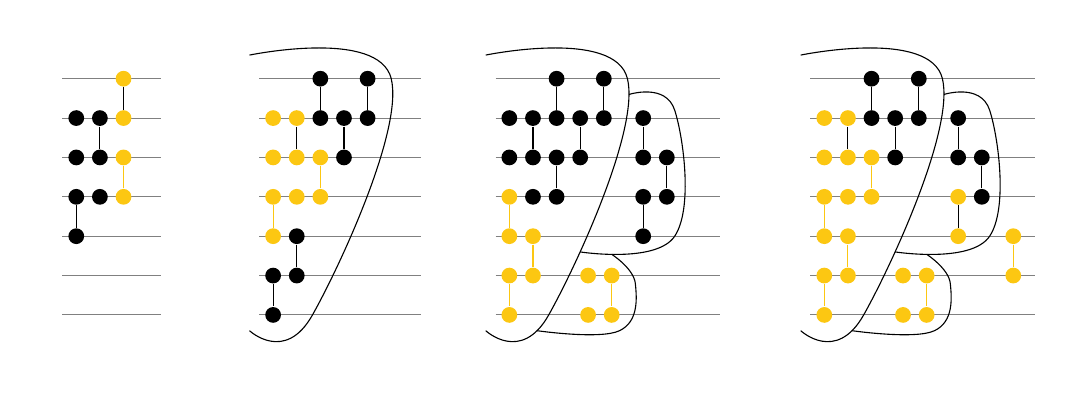
\begin{tikzpicture}
\begin{scope}[scale=1]

\newcommand{\eeee}{mycolor}
\newcommand{\eeeeee}{mycolor}
\newcommand{\eeeee}{1.5cm}
\newcommand{\vfour}{black}
\newcommand{\vfourr}{mycolor}
\newcommand{\colw}{black}
\newcommand{\spec}{\vfour}
\newcommand{\ff}[1]{{}}

\newcommand{\ssss}{
\tikzstyle{every node}=[node distance=.5cm]
\node(lab1) at (1,-1) { };
\node(lab2) [below of=lab1] { };
\node(lab3) [below of=lab2] { };
\node(lab4) [below of=lab3] { };
\node(lab5) [below of=lab4] { };
\node(lab6) [below of=lab5] { };
\node(lab7) [below of=lab6] { };
\tikzstyle{every node}=[node distance=.2cm]
\node(l1) [right of=lab1] {};
\tikzstyle{every node}=[node distance=.5cm]
\node(l2) [below of=l1] {};
\node(l3) [below of=l2] {};
\node(l4) [below of=l3] {};
\node(l5) [below of=l4] {};
\node(l6) [below of=l5] {};
\node(l7) [below of=l6] {};
\tikzstyle{every node}=[node distance=\eeeee]
\node(r1) [right of=l1] {};
\draw[gray] (l1) -- (r1);
\node(r2) [right of=l2] {};
\draw[gray] (l2) -- (r2);
\node(r3) [right of=l3] {};
\draw[gray] (l3) -- (r3);
\node(r4) [right of=l4] {};
\draw[gray] (l4) -- (r4);
\node(r5) [right of=l5] {};
\draw[gray] (l5) -- (r5);
\node(r6) [right of=l6] {};
\draw[gray] (l6) -- (r6);
\node(r7) [right of=l7] {};
\draw[gray] (l7) -- (r7);

\tikzstyle{every state}=[fill=black,draw=none,inner sep=0pt,minimum size=0.2cm]
\tikzstyle{every node}=[node distance=.3cm]
\node[state](a2)[right of=l2, fill=\vfour]{};
\tikzstyle{every node}=[node distance=.5cm]
\node[state](a3)[below of=a2, fill=\vfour]{};
\node[state](a4)[below of=a3, fill=\spec]{};
\node[state](a5)[below of=a4, fill=\spec]{};
\draw[\spec] (a4) -- (a5);
\ff{\node[state](a6)[below of=a5, fill=\colw]{};
\node[state](a7)[below of=a6, fill=\colw]{};
\draw[\colw] (a6) -- (a7);}

\node[state](b2)[right of=a2, node distance=.3cm, fill=\vfour]{};
\node[state](b3)[below of=b2, fill=\vfour]{};
\draw (b2) -- (b3);
\node[state](b4)[below of=b3, fill=\vfour]{};
\ff{\node[state](b5)[below of=b4, fill=\eeeeee]{};
\node[state](b6)[below of=b5, fill=\eeeeee]{};
\draw[color=\eeeeee] (b5) -- (b6);
}

\node[state](c2)[right of=b2, fill=\eeee, node distance=.3cm]{};
\node[state](c1)[above of=c2, fill=\eeee]{};
\draw (c1) -- (c2);
\node[state](c3)[below of=c2, fill=\vfourr]{};
\node[state](c4)[below of=c3, fill=\vfourr]{};
\draw[\vfourr] (c3) -- (c4);

\ff{
\node[state](d2)[right of=c2, node distance=.3cm]{};
\node[state](d3)[below of=d2]{};
\draw (d2) -- (d3);

\node[state](e2)[right of=d2, node distance=.3cm, fill=\eeee]{};
\node[state](e1)[above of=e2, fill=\eeee]{};
\draw[color=\eeee] (e2) -- (e1);

\node(u)[above right of=e1]{};

\draw [black] plot [smooth, tension=0.7] coordinates { (1.2,-0.7) (3,-1) (2,-4) (1.2,-4.2)};
}
}


\ssss

\renewcommand{\eeee}{black}
\renewcommand{\eeeee}{2.3cm}
\renewcommand{\vfour}{mycolor}
\renewcommand{\vfourr}{\vfour}
\renewcommand{\eeeeee}{black}
\renewcommand{\ff}[1]{{#1}}

\begin{scope}[shift={(2.5,0)}]
\ssss
\node(view)[right of =c4, node distance=0.8cm]{\color{\vfour}};
\end{scope}

\renewcommand{\eeeee}{3.1cm}
\renewcommand{\vfour}{black}
\newcommand{\colv}{black}
\renewcommand{\colw}{mycolor}
\renewcommand{\spec}{\colw}
\renewcommand{\eeeeee}{\colw}
\newcommand{\eeeeeeee}{black}

\newcommand{\sssss}{
\ssss
\node[state](f2)[right of =e2,fill=\colv]{};
\node[state](f3)[below of =f2,fill=\colv]{};
\draw[\colv] (f2)--(f3);
\node[state](f4)[below of =f3,fill=\eeeeeeee]{};
\node[state](f5)[below of =f4,fill=\eeeeeeee]{};
\draw[\colv] (f4)--(f5);
\node[state](g3)[right of =f3, node distance=.3cm]{};
\node[state](g4)[below of =g3]{};
\draw[\colv] (g3)--(g4);

\node(v)[above right of =g3]{};
\draw [black] plot [smooth, tension=0.7] coordinates { (3.02,-1.2) (3.6,-1.4) (3.6,-3) (2.4,-3.2)};


\node[state](d6)
[right of =b6,fill=\colw, node distance=.7cm]{};
\node[state](d7)
[below of =d6,fill=\colw]{};
\node[state](e6)
[right of =d6,fill=\colw, node distance=.3cm]{};
\node[state](e7)
[below of =e6,fill=\colw]{};
\draw[\colw] (e6)--(e7);
\node(w)
[right of =e6, node distance=.5cm]{};


\draw [black] plot [smooth, tension=0.7] coordinates { (2.8,-3.23) (3.1,-3.6) (2.9,-4.2) (1.85,-4.2)};
}

\begin{scope}[shift={(5.5,0)}]
\sssss


\node(view)[right of =e7, node distance=1cm]{\color{\colw}};

\end{scope}

\renewcommand{\eeeee}{3.1cm}
\renewcommand{\vfour}{mycolor}
\renewcommand{\colv}{black}
\renewcommand{\colw}{mycolor}
\renewcommand{\spec}{mycolor}
\renewcommand{\eeeeee}{mycolor}
\renewcommand{\eeeeeeee}{mycolor}

\begin{scope}[shift={(9.5,0)}]
\sssss

\node[state](oups)[right of =f5, node distance=.7cm, fill=mycolor]{};
\node(c)[below right of =oups, node distance=.3cm]{};
\node[state](oups2)[below of =oups, fill=mycolor]{};
\draw[mycolor] (oups)--(oups2);

\node(w)
[below right of =oups2, node distance=.5cm]{ \color{mycolor}};

\end{scope}

\end{scope}
\end{tikzpicture}


\caption{\label{fig:example}
The set processes is .
A letter is identified with its domain.
Here the domains are either singletons, represented by a single dot,
or pairs of contigous processes,
represented by two dots connected with a vertical segment.
On the left handside is represented the trace

which has two maximal letters  and  thus is not prime.
Center left: process  sees only its causal view  (in yellow).
Center right:  since . Both  and  (in yellow) are prime prefixes of  and they are parallel.
Right:  and  (in yellow) are parallel.
}
\end{figure}

\paragraph*{Processes and automata}



Asynchronous automata are to traces what finite automata are to finite words, as witnessed by Zielonka's theorem~\cite{zautomata}. An asynchronous automaton is a collection of automata on finite words, whose transition tables do synchronize on certain actions. 



\begin{definition}
An asynchronous automaton on alphabet  with processes  is a tuple

where:
\begin{itemize}
\item
 every process  has a set of actions
 , a set of states 
 and  is the initial state of  and  its set of final states.
\item
 .
 For every letter , the domain of  is 
 
 \item
 is a set of transitions of the form 

where 
and .
Transitions are \emph{deterministic}: for every ,
if

and 
then 
(hence 
 ).
\end{itemize}
\end{definition}

Such an automaton works asynchronously:
each time a letter  is processed, the states of the processes
in  are updated according to the corresponding
transition, while the states of other processes do not change.
This induces a natural commutation relation  on :
two letters commute iff they have no process in common i.e.


The set of \emph{plays} of the automaton 
is a set of traces denoted  and defined inductively, along with 
a mapping .
\begin{itemize}
\item  is a play and ,
\item for every play  such that  is defined
and 
is a transition then
 is a play and
p\not\in\dom(a)
\end{itemize}

For every play ,  is called the \emph{global state} of .
The inductive definition of  is correct because it is invariant by
commutation of independent letters of .


\paragraph*{Counting actions of a process}
For every trace  we can count how many times a process 
has played an action in , which we denote .
Formally,  is first defined for words, as the length of the projection
of  on , which is invariant by commuting letters.
The domain of a trace is defined as 


\paragraph*{Views, strategies and games}

Given an automaton ,
we want the processes to choose actions
which guarantee that
every play eventually terminates in a final state.

To take into account the fact that some actions are controllable by processes while some other actions are not, we assume that  is partitioned in 

where  is the set of controllable actions and
 the set of (uncontrollable)  environment actions.
Intuitively, processes cannot prevent their environment to 
play actions in , while they can decide whether to block or allow any action in .

We adopt a modern terminology and call the automaton  together with the partition
 a \emph{distributed game}, or even more simply a \emph{game}.
In this game the processes play distributed strategies,
which are individual plans of action for each process.
The choice of actions by a process  is dynamic: at every step,  chooses a new set of controllable actions, depending on its  information about the way the play is going on. This information is limited since
processes cannot communicate together unless they synchronize on a
common action. In that case however they exchange as much information about the play as they want.
Finally, the information missing to a process is the set of actions which happened in parallel of its own actions.
The information which remains is called the -view of the play,
and is defined formally as follows.







\begin{definition}[Views]\label{def:views}
For every set of processes 
and trace ,
the \emph{-view} of , denoted ,
 is the unique trace such that
  factorizes as
 and
 is the longest suffix of  such that 
.
In case  is a singleton  the view is denoted
 and is a prime trace.
For every letter  we denote .
\end{definition}

The well-definedness of the -view is shown in the appendix, where we also establish:


We can now define what is a distributed strategy.

\begin{definition}[Distributed strategies, consistent and maximal plays]
Let  be a distributed game.
A \emph{strategy for process } in  is a mapping
which associates with every play  a set of actions  such that:
\begin{itemize}
\item
environment actions are allowed: ,
\item
the decision depends only on the view of the process:
.
\end{itemize}
A \emph{distributed strategy}
 is a tuple 
where each  is a strategy of process .
A play  is \emph{consistent with },
or equivalently is a \emph{-play} if:

A -play is \emph{maximal} if it is not the strict prefix of another -play.
\end{definition}

Note that a strategy is forced to allow every environment action to be executed at every moment.
This may seem to be a huge strategic advantage for the environment.
However depending on the current state,
not every action can be effectively used in a transition
because the transition function is not assumed to be total.
So in general not every environment actions can actually occur in a play.
In particular it may happen that a process enters a final state
with no outgoing transition, where
no uncontrollable action can happen.
 
 \paragraph*{Winning games}
 
Our goal is to synthesize  strategies
which ensure that the game terminates and 
all processes are in a final state.

\begin{definition}[Winning strategy]
A strategy  is winning if
the set of -plays  is finite
and in every maximal -play ,
every process is in a final state
i.e. 
\end{definition}
We are interested in the following problem, whose decidability is an open question.
\smallskip

{\noindent \sc Distributed synthesis problem:}
given a distributed game decide
whether  there exists a winning strategy.

\smallskip

If the answer is positive,
the algorithm should as well compute a
winning strategy.




\section{Three decidable classes}
\label{sec:examples}

\paragraph*{Series-parallel games}
A game is \emph{series-parallel} if its dependency alphabet 
is a co-graph i.e. belongs to the smallest class of graphs containing singletons and closed under parallel product and complementation. In this case  has a \emph{decomposition tree},
this is a binary tree whose nodes are subsets of ,
its leaves are the singletons ,
its root is .
Moreover
every node  with two children  and 
 is the disjoint union of  and 
 and either 
 
(serial product)
 or   (parallel product).

The synthesis problem is decidable for series-parallel games~\cite{gastin}.


 
\paragraph*{Connectedly communicating games}
A game is \emph{-connectedly communicating}  if
for every pair  of processes,
 if process  plays  times in parallel of process 
 then all further actions of  will be parallel to .
 Formally, for every prime play ,



The MSO theory of the event structure
of a -connectedly communicating game is decidable~\cite{madhu},
which implies that controller synthesis is decidable for theses games.




\paragraph*{Acyclic games}
An acyclic game is a game where processes  are the nodes of a tree 
and the domain of every action is a connected set of nodes of .
The synthesis problem is known to be decidable
for acyclic games such that the domain of each action has size  or ~\cite{acyclic}.


\section{Simplifying strategies}
\label{sec:simplifying}

In this section we present an elementary operation called a \emph{shortcut},
which can be used to simplify and reduce the duration of a winning strategy.

To create a shortcut, one selects a -play 
and modify the strategy  so that as soon as any of the processes
sees the play  in its view, this process assumes that not only  but also  has actually occurred.
In other words, a shortcut is a kind of \emph{cut-and-paste} in the strategy:
we glue on node  the sub-strategy rooted at node .

The choice of  and  should be carefully performed so that 
the result of the shortcut
is still a strategy.
We provide a sufficient condition for that:  should be a  \emph{useless repetition}.

The interest of taking shortcuts is the following:
if the original strategy is winning,
then the  strategy obtained by taking the shortcut
is winning as well,
and strictly smaller than the original one.
In the remainder of this section, we formalize these concepts.



\subsection{Locks}

We need to limit the communication between a set of processes,
called a team, and processes outside the team.
This leads to the notion of a -lock:
this is a prime play 
such that there is no synchronization  between  and  in parallel of .




\begin{definition}
Let .
An action  is -safe if .
A play  is a \emph{-lock} 
if it is prime and the last action of every prime play parallel to  is -safe.
\end{definition}


\iffalse

\begin{figure}


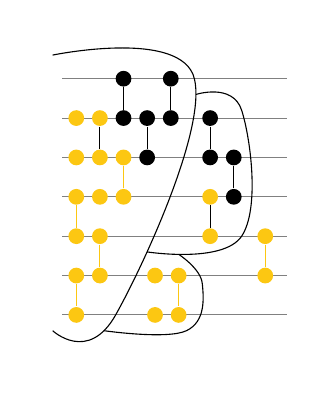
\begin{tikzpicture}
\begin{scope}[scale=1]

\newcommand{\eeee}{mycolor}
\newcommand{\eeeeee}{mycolor}
\newcommand{\eeeee}{1.5cm}
\newcommand{\vfour}{black}
\newcommand{\vfourr}{mycolor}
\newcommand{\colw}{black}
\newcommand{\spec}{\vfour}
\newcommand{\ff}[1]{{}}

\newcommand{\ssss}{
\tikzstyle{every node}=[node distance=.5cm]
\node(lab1) at (1,-1) { };
\node(lab2) [below of=lab1] { };
\node(lab3) [below of=lab2] { };
\node(lab4) [below of=lab3] { };
\node(lab5) [below of=lab4] { };
\node(lab6) [below of=lab5] { };
\node(lab7) [below of=lab6] { };
\tikzstyle{every node}=[node distance=.2cm]
\node(l1) [right of=lab1] {};
\tikzstyle{every node}=[node distance=.5cm]
\node(l2) [below of=l1] {};
\node(l3) [below of=l2] {};
\node(l4) [below of=l3] {};
\node(l5) [below of=l4] {};
\node(l6) [below of=l5] {};
\node(l7) [below of=l6] {};
\tikzstyle{every node}=[node distance=\eeeee]
\node(r1) [right of=l1] {};
\draw[gray] (l1) -- (r1);
\node(r2) [right of=l2] {};
\draw[gray] (l2) -- (r2);
\node(r3) [right of=l3] {};
\draw[gray] (l3) -- (r3);
\node(r4) [right of=l4] {};
\draw[gray] (l4) -- (r4);
\node(r5) [right of=l5] {};
\draw[gray] (l5) -- (r5);
\node(r6) [right of=l6] {};
\draw[gray] (l6) -- (r6);
\node(r7) [right of=l7] {};
\draw[gray] (l7) -- (r7);

\tikzstyle{every state}=[fill=black,draw=none,inner sep=0pt,minimum size=0.2cm]
\tikzstyle{every node}=[node distance=.3cm]
\node[state](a2)[right of=l2, fill=\vfour]{};
\tikzstyle{every node}=[node distance=.5cm]
\node[state](a3)[below of=a2, fill=\vfour]{};
\node[state](a4)[below of=a3, fill=\spec]{};
\node[state](a5)[below of=a4, fill=\spec]{};
\draw[\spec] (a4) -- (a5);
\ff{\node[state](a6)[below of=a5, fill=\colw]{};
\node[state](a7)[below of=a6, fill=\colw]{};
\draw[\colw] (a6) -- (a7);}

\node[state](b2)[right of=a2, node distance=.3cm, fill=\vfour]{};
\node[state](b3)[below of=b2, fill=\vfour]{};
\draw (b2) -- (b3);
\node[state](b4)[below of=b3, fill=\vfour]{};
\ff{\node[state](b5)[below of=b4, fill=\eeeeee]{};
\node[state](b6)[below of=b5, fill=\eeeeee]{};
\draw[color=\eeeeee] (b5) -- (b6);
}

\node[state](c2)[right of=b2, fill=\eeee, node distance=.3cm]{};
\node[state](c1)[above of=c2, fill=\eeee]{};
\draw (c1) -- (c2);
\node[state](c3)[below of=c2, fill=\vfourr]{};
\node[state](c4)[below of=c3, fill=\vfourr]{};
\draw[\vfourr] (c3) -- (c4);

\ff{
\node[state](d2)[right of=c2, node distance=.3cm]{};
\node[state](d3)[below of=d2]{};
\draw (d2) -- (d3);

\node[state](e2)[right of=d2, node distance=.3cm, fill=\eeee]{};
\node[state](e1)[above of=e2, fill=\eeee]{};
\draw[color=\eeee] (e2) -- (e1);

\node(u)[above right of=e1]{};

\draw [black] plot [smooth, tension=0.7] coordinates { (1.2,-0.7) (3,-1) (2,-4) (1.2,-4.2)};
}
}

\renewcommand{\eeee}{black}
\renewcommand{\eeeee}{2.3cm}
\renewcommand{\vfour}{mycolor}
\renewcommand{\vfourr}{\vfour}
\renewcommand{\eeeeee}{black}
\renewcommand{\ff}[1]{{#1}}
\renewcommand{\eeeee}{3.1cm}
\renewcommand{\vfour}{black}
\newcommand{\colv}{black}
\renewcommand{\colw}{mycolor}
\renewcommand{\spec}{\colw}
\renewcommand{\eeeeee}{\colw}
\newcommand{\eeeeeeee}{black}

\newcommand{\sssss}{
\ssss
\node[state](f2)[right of =e2,fill=\colv]{};
\node[state](f3)[below of =f2,fill=\colv]{};
\draw[\colv] (f2)--(f3);
\node[state](f4)[below of =f3,fill=\eeeeeeee]{};
\node[state](f5)[below of =f4,fill=\eeeeeeee]{};
\draw[\colv] (f4)--(f5);
\node[state](g3)[right of =f3, node distance=.3cm]{};
\node[state](g4)[below of =g3]{};
\draw[\colv] (g3)--(g4);

\node(v)[above right of =g3]{};
\draw [black] plot [smooth, tension=0.7] coordinates { (3.02,-1.2) (3.6,-1.4) (3.6,-3) (2.4,-3.2)};


\node[state](d6)
[right of =b6,fill=\colw, node distance=.7cm]{};
\node[state](d7)
[below of =d6,fill=\colw]{};
\node[state](e6)
[right of =d6,fill=\colw, node distance=.3cm]{};
\node[state](e7)
[below of =e6,fill=\colw]{};
\draw[\colw] (e6)--(e7);
\node(w)
[right of =e6, node distance=.5cm]{};


\draw [black] plot [smooth, tension=0.7] coordinates { (2.8,-3.23) (3.1,-3.6) (2.9,-4.2) (1.85,-4.2)};
}

\renewcommand{\eeeee}{3.1cm}
\renewcommand{\vfour}{mycolor}
\renewcommand{\colv}{black}
\renewcommand{\colw}{mycolor}
\renewcommand{\spec}{mycolor}
\renewcommand{\eeeeee}{mycolor}
\renewcommand{\eeeeeeee}{mycolor}

\begin{scope}[shift={(10,0)}]
\sssss

\node[state](oups)[right of =f5, node distance=.7cm, fill=mycolor]{};
\node(c)[below right of =oups, node distance=.3cm]{};
\node[state](oups2)[below of =oups, fill=mycolor]{};
\draw[mycolor] (oups)--(oups2);

\node(w)
[below right of =oups2, node distance=.5cm]{ \color{mycolor}};

\end{scope}

\end{scope}
\end{tikzpicture}
\caption{\label{fig:lock}
 and  (in yellow) are parallel.
}
\end{figure}
\fi

The notion of lock is illustrated on
the right handside of Fig.~\ref{fig:example}.
Set .
Then
 is not a -lock because 
 is parallel to 
but  is
not -safe.
Locks occur in a variety of situations,
including the three decidable classes.


\begin{lemma}[Sufficient conditions for -locks]
\label{lem:lock}
Let  be a prime play of a game  and .
Each of the following conditions is sufficient for  to be a -lock:
\begin{itemize}
\item[i)]
.
\item[ii)]
  is a -lock.
\item[iii)]
.
\item[iv)]
The game is series-parallel and 
where  is the smallest node of the decomposition tree of  which contains
.
\item[v)]
The game is connectedly communicating game with bound ,  and .
\item[vi)]
The game is acyclic with respect to a tree 
and  is the set of descendants in 
of the processes in .
\item[vii)]
There are two traces  and  such that  and   is a -lock
in the game  identical to  except  the initial state is changed to .
\end{itemize}
\end{lemma}







\subsection{Taking shortcuts}

In this section we present a basic operation
used to simplify a strategy, called a \emph{shortcut},
which consists in modifying certain parts of a strategy,
called \emph{useless repetitions}.
These notions rely on the notion of \emph{strategic state} as well as two operations on strategies called \emph{shifting} and \emph{projection}.

\begin{definition}[Residual]
Let  be a strategy,
 a -play and .
The -residual of  after  is
the set:

\end{definition}

A winning strategy may take unnecessarily complicated detours in order to ensure termination.
Such detours are called \emph{useless repetitions}.
\begin{definition}[Strategic state]
Let  be a state of processes,
 a strategy and  a prime -play with maximal letter .
The strategic -state of  after  is the tuple


\end{definition}






\begin{definition}[Useless repetition]
A useless -repetition in a strategy 
is a pair of traces  such that  is not empty,
 is a -play,  ,
both  and  are -locks and .
\end{definition}

The following theorem is the key to our decidability results.

\begin{theorem}
If there exists a winning strategy
then there exists a winning strategy 
without any useless repetition.
\label{theo:uselessdistrib}
\end{theorem}

The proof of this theorem relies on the notion of shortcuts,
an operation which turns a winning strategy into another strategy with strictly shorter duration.

\begin{definition}[Duration of a strategy]
The duration of a strategy  is 

\end{definition}

The duration of a  strategy  may in general be infinite but is finite if  is winning.

\begin{lemma}
\label{lem:shortcut}
Let  be a  useless -repetition in a  strategy .
Let  and  defined by

and

Then  is a strategy
called the \emph{-shortcut of }.
Moreover
for every trace ,
\be
\label{eq:tauplay}
(\text{ is a -play})
\iff 
(\text{ is a -play})
\enspace.
\ee
If  is a winning strategy then  is winning as well and has a strictly smaller duration.
\end{lemma}
\begin{proof}[Sketch of proof of Lemma~\ref{lem:shortcut}]
The full proof can be found in the appendix.
That  is a strategy follows from the definition:  only depends on . To establish~\eqref{eq:tauplay},
the central point is to show that for every -play ,

There are three types of plays depending whether:
\begin{enumerate}
\item
 has not occurred  (),
\item
 has occurred in parallel of the process 
(),
\item
 knows that
 has occurred
().
\end{enumerate}
It may happen that  and
there exists a process  in case 2 and a process  in case 3. Then process  is playing the modified strategy
 while process  is still playing the original strategy , which may \emph{a priori} create some -plays unrelated with .
The equality of the strategic states in  and  ensures that the equivalence~\eqref{eq:tauplay} stays valid.

Moreover, thanks to~\eqref{eq:tauplay},
 implies  because  is not empty.
And according to~\eqref{eq:tauplay} again,
the set of global states of the maximal plays is the same for  and  thus if  is winning then  is winning as well.
\end{proof}

\begin{proof}[Proof of Theorem~\ref{theo:uselessdistrib}]
As long as there exists a useless repetition,
take the corresponding shortcut.
According to Lemma~\ref{lem:shortcut},
this creates a sequence 
of winning strategies whose duration strictly decreases. Thus the sequence is finite and its last element
is a winning strategy without useless repetition.
\end{proof}



\section{Decomposable games}
\label{sec:decomposable}

In this section we introduce \emph{decomposable} games,
for which the \dsp\ is decidable (Theorem~\ref{theo:dec}).
There are actually three notions of decomposability:
structural decomposability, process decomposability and action decomposability.
These three notions form a hierarchy:
structural decomposability implies process decomposability which itself implies action decomposability (Lemma~\ref{lem:hier}).
Known decidable classes are decomposable:
acyclic games are structurally decomposable (Lemma~\ref{lem:acyclic}),
connectedly-communicating games are process decomposable (Lemma~\ref{lem:pdec})
and series-parallel games are action decomposable
(Lemma~\ref{lem:adec}).
Structural decomposability is stable under some  operations between games which leads to new examples
of decidable games (Lemma~\ref{lem:merging}).

\subsection{Decomposability}



The notions of decomposability rely on \emph{preorders} defined on  or . A preorder  is a reflexive and transitive relation.
We denote  the relation .
 
\paragraph*{Structural decomposability}
The notion of structural decomposability relies on a preorder
 on  
which is 
monotonic with respect to inclusion, i.e. ,
.



\begin{definition}[Structural decomposability]
\label{unif}
A game is \emph{-structurally decomposable}
if for every non-empty prime trace 
there exists 
and  
such that:

\end{definition}

We have already seen one example of structurally decomposable game.

\begin{lemma}\label{lem:acyclic}
Acyclic games are structurally decomposable.
\end{lemma}
\begin{proof}
Assume the game is acyclic with process tree .
Set 
 iff 
every process in  has a -ancestor in , which is  monotonic with respect to inclusion.
Let  be a prime trace,
 the least common ancestor
in  of processes in  and  the set of descendants of .
Then .
Moreover, since  is prime and since the domain of every action is a connected subset of 
then  is connected as well thus 
and there exists a letter  such that .
We show that  satisfies the conditions in the definition of structural decomposability.
First, 
and the inequality is strict because 
the only ancestor of  in  is  itself and .
Second, let  such that .
Then  and since  is connected in ,
then either none of the processes in  or
all of them are descendants of  in , i.e.  is -safe.
\end{proof}




\paragraph*{Process decomposability}


The definition of process decomposable games relies on
a parameter  and a preorder  on 
which is 
monotonic with respect to inclusion.


\begin{definition}[Process decomposable games]
Fix an integer .
A trace  is \emph{-repeating} if 

A game is \emph{-process decomposable}
if  for every prime play ,
if  is -repeating then
there exists 
and a prime prefix 
such that 
 is a  -lock 
and 

\end{definition}

We have already seen one example of process decomposable games.

\begin{lemma}\label{lem:pdec}
Connectedly communicating games
are process decomposable.
\end{lemma}


\paragraph*{Action decomposability}

\newcommand{\FF}{\mathcal{F}}

\newcommand{\dFF}{{\downarrow\FF}}














Action decomposability is defined with respect to a parameter 
and a preorder  on 
which is 
monotonic with respect to inclusion.

\begin{definition}[Action decomposable games]
Let  be an integer.
A game is \emph{ action decomposable}
if  for every prime play 
such that
 is -repeating,
there exists 
and a prime prefix  such that 
 is a  -lock
and

\end{definition}



We have already seen one example of action decomposable games.

\begin{lemma}\label{lem:adec}
Series-parallel games
are action decomposable.
\end{lemma}





\paragraph*{A hierarchy}


\begin{lemma}\label{lem:hier}
Every structurally decomposable game is process decomposable
and every process decomposable game is action decomposable.
\end{lemma}

Thus \emph{action decomposability} is the most general notion
of decomposability.
In the sequel for the sake of conciseness,
it is simply called \emph{decomposability}.


\subsection{Decidability}
In this section we show that decomposability is a decidable property
and decomposable games have a decidable controller synthesis problem.




\begin{lemma}[Decomposability is decidable]
\label{decdec}
 Whether a game is decomposable is decidable.
There exists a computable function 
from games to integers
such that whenever a game 
is  decomposable
 for some , it is  decomposable.
 \end{lemma}
 The proof is elementary and can be found in the appendix.




\begin{theorem}\label{theo:dec}
The distributed synthesis problem is decidable for decomposable games.
\end{theorem}



\begin{proof}[Proof of Theorem~\ref{theo:dec}]
\newcommand{\CC}{\mathcal{C}}

We show that there exists a computable function 
from games to integers
such that in every decomposable distributed game 
every strategy with no useless repetition
has duration .

Let  be a preorder on  compatible with inclusion,
 an integer and 
 a  action decomposable distributed game.
Assume  w.l.o.g. (cf. Lemma~\ref{decdec}).

For every set of actions ,
denote  the game with  actions 
and the same processes, initial state and final states than .
The transitions of  are all transitions of  whose
 action is in . An action  is controllable in  iff it is controllable in .


We show that for every  the game  is  decomposable,
where  denotes the restriction of  to . Let  be a prime play of  
such that  is -repeating.
Since   is  decomposable, there exists
 and a prime prefix 
such that  is a  -lock in 
and 
where
a \ind \last(z).
Since  is monotonic with respect to inclusion
 then b\ind \last(z)
 thus
 .
 Since  is a play in  then  is a play in  as well.
 And since every play in  is a play in ,  is a  -lock not only in  but also in .
All conditions of action decomposability are met :
   is  decomposable.


\medskip

Denote   the largest size of a complete undirected graph whose edges are labelled with  
and which contains no monochromatic clique of size .
According to Ramsey theorem,
 is finite and computable. 
For every ,
defined inductively  as
:

with the convention .

Fix a strategy  with no useless repetition.
We prove that for every  -play ,

The proof is by induction on  with respect to .
The base case when 
is easy, in this case
.


Now let  be a -play consistent with .
Assume the induction hypothesis holds: for every -play , if

then
 . 
 
 We start with computing,
for every non-empty set of letters  
an upper bound on the length of every factorization

such that

For a start, we consider the case where  is connected in the sense
where the dependency graph  is connected.
Set .
For ,
denote 
 the concatenation

and 
.
Let  and fix some .

Let 
.
We show that  is -repeating
and .
Since
,
according to property~\eqref{eq:viewdec}
of views
there exists a sequence 
 such that

where  and for every ,
.
Since the sequence
 is monotonic,
there exists 
such that .
Denote 
and 
and
.
By definition of views,
and according to~\eqref{eq:alphabets},
. Since  and  then

thus . Since  then finally .
Thus the set  is a connected component of the graph :
by definition of  and , all edges with source  have target in .
However by hypothesis  is connected thus 
and .
Finally  and since ,
the sequence  is constant equal to .
Thus, according to~\eqref{eq:alphabets} and the definition of ,
for every ,
.
Thus, according to~\eqref{eq:alphabets} and~\eqref{eqfacto}
and since ,
every letter of  occurs at least  times in 
thus
 is -repeating and .

Since the game is 
decomposable
and  is -repeating,
and
,
there exists
a superset  of ,
an action ,
and a prime prefix 
such that
the play

is a -lock
and
\newcommand{\Tl}{\TT^{(\ell)}}


For every ,
denote

the  strategic state of  after .
We show two properties of .
\begin{itemize}
\item
First, all elements of  are distinct.
For the sake of contradiction, assume 
for some .
We show that .
Since  then  , denote this letter .
Then

where the second inequality holds
because

since ,
and the third inequality holds because 
thus  hence property~\eqref{viewsub} applies.
Moreover the last inequality is strict because there is at least one more  in
 than in .
We get a contradiction because by hypothesis there is no useless repetition in ,
however, denoting  and  such that ,
the pair  is a useless -repetition in :
by hypothesis the strategic -states of  and  are equal and both  and  are -locks, moreover  is not empty because 
and finally .
Thus  is a useless repetition in .
\item
Second, for every , 
all plays in  have length .
Let  be a -play such that .
Then .
Since  is monotonic with respect to inclusion,

Thus by induction hypothesis,
.
\end{itemize}

According to the second property,
there
are at most  different residuals appearing in the sequence
.
Thus the sequence  takes at most 

different values.
And according to the first property, all these states are different thus 
.

The inequality  has been established  under the assumption that  is connected.
The general case reduces to this case: let 
be a connected component of  and for 
let  be the projection of  on .
Then 
and
there exists  such that
 thus .



Let us reformulate the inequality  as a property of an undirected complete graph
with edges colored by .
Let  the factorization of  into its letters.
Let  be the complete graph with vertices 
and the label of the edge  with  is the set of letters .
Then every  monochromatic clique of  has size .
Thus, according to Ramsey theorem,
,
which completes the inductive step.

As a consequence, winning strategies in  can be looked for in the finite family of strategies
whose all plays have length 
with  computable.
As a consequence,
the synthesis problem
can be solved
by enumerating all these strategies and testing whether any of them is winning.
For testing whether a strategy of finite duration
is winning the algorithm simply checks that the global state of all the maximal plays is final.
\end{proof}



\subsection{New examples of decidable games}

The three classes of games whose decidability is already known
are decomposable  (cf Lemmas~\ref{lem:acyclic},~\ref{lem:pdec} and~\ref{lem:adec}).
In this section we give some new examples of decidable games.


\begin{lemma}\label{lem:fourp}
Four players games are  structurally decomposable.
\end{lemma}

Although our techniques do not seem to provide an algorithm for solving games with five processes, they can address a special case of those.

\begin{lemma}\label{lem:fivep}
Let  be a distributed game with five processes.
Assume that the number of actions
that a process can successively play in a row without 
synchronizing simultaneously with two other processes
is bounded.
Then  is process decomposable.
\end{lemma}

Another decidable example is the class of \emph{majority games}:
\begin{lemma}[Majority games]\label{lem:majority}
Assume that every non-local action synchronizes a majority of the processes i.e. for every action ,

Then the game is  structurally decomposable.
\end{lemma}












The class of structurally decomposable games
is stable under projection and merge.

\begin{definition}[Projecting games]
Let  be a game with processes  and
alphabet .
Let 

a subset of the processes.
The projection of  on  is the game 
with processes  and alphabet

partitioned in .
The states of a process  are the same in  and , every transition 

of  on a letter 
is projected to ,
and every transition on a letter  is simply deleted.
\end{definition}

The following result combines two structurally decomposable games into one.


\begin{lemma}[Merging games]\label{lem:merging}
Let  be a game,
and 
 two set of processes such that  and for every action ,

If both projections of  on  and  are structurally decomposable then  is structurally decomposable.
\end{lemma}

The merge operation can combine two structurally decomposable games in order to create a new one.
For example all acyclic games can be obtained this way,
since -player games are structurally decomposable
and every tree with more than three 
nodes
can be obtained by merging two strictly smaller subtrees.
This technique can go beyond acyclic games,
by merging together 4-player games
and majority games.
The graph of processes is an undirected graph with nodes 
 and there is an edge between  and 
whenever both  and  both belong to the domain of one of the actions.
Then all the games whose graph of processes
is contained in the one depicted on Fig.~\ref{fig:network} are structurally decomposable.



\begin{figure}[ht]
\begin{center}
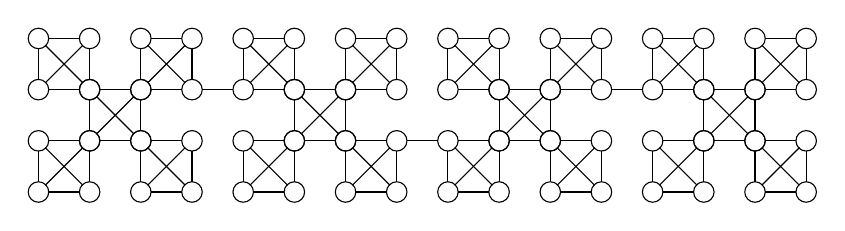
\begin{tikzpicture}
\begin{scope}[scale=1.3]

\begin{scope}
\draw (0,0) circle (0.1);
\draw (0.5,0) circle (0.1);
\draw (0.5,0.5) circle (0.1);
\draw (0,0.5) circle (0.1);
\draw (0.1,0) -- (0.4,0) ;
\draw (0,0.1) -- (0,0.4) ;
\draw (0.1,0.5) -- (0.4,0.5) ;
\draw (0.5,0.4) -- (0.5,0.1) ;
\draw (0.065,0.065) -- (0.435,0.435) ;
\draw (0.065,0.435) -- (0.435,0.065) ;
\end{scope}

\begin{scope}[shift={(0.5,0.5)}]
\draw (0,0) circle (0.1);
\draw (0.5,0) circle (0.1);
\draw (0.5,0.5) circle (0.1);
\draw (0,0.5) circle (0.1);
\draw (0.1,0) -- (0.4,0) ;
\draw (0,0.1) -- (0,0.4) ;
\draw (0.1,0.5) -- (0.4,0.5) ;
\draw (0.5,0.4) -- (0.5,0.1) ;
\draw (0.065,0.065) -- (0.435,0.435) ;
\draw (0.065,0.435) -- (0.435,0.065) ;
\end{scope}

\begin{scope}[shift={(-0.5,0.5)}]
\draw (0,0) circle (0.1);
\draw (0.5,0) circle (0.1);
\draw (0.5,0.5) circle (0.1);
\draw (0,0.5) circle (0.1);
\draw (0.1,0) -- (0.4,0) ;
\draw (0,0.1) -- (0,0.4) ;
\draw (0.1,0.5) -- (0.4,0.5) ;
\draw (0.5,0.4) -- (0.5,0.1) ;
\draw (0.065,0.065) -- (0.435,0.435) ;
\draw (0.065,0.435) -- (0.435,0.065) ;
\end{scope}

\begin{scope}[shift={(-0.5,-0.5)}]
\draw (0,0) circle (0.1);
\draw (0.5,0) circle (0.1);
\draw (0.5,0.5) circle (0.1);
\draw (0,0.5) circle (0.1);
\draw (0.1,0) -- (0.4,0) ;
\draw (0,0.1) -- (0,0.4) ;
\draw (0.1,0.5) -- (0.4,0.5) ;
\draw (0.5,0.4) -- (0.5,0.1) ;
\draw (0.065,0.065) -- (0.435,0.435) ;
\draw (0.065,0.435) -- (0.435,0.065) ;
\end{scope}

\begin{scope}[shift={(0.5,-0.5)}]
\draw (0,0) circle (0.1);
\draw (0.5,0) circle (0.1);
\draw (0.5,0.5) circle (0.1);
\draw (0,0.5) circle (0.1);
\draw (0.1,0) -- (0.4,0) ;
\draw (0,0.1) -- (0,0.4) ;
\draw (0.1,0.5) -- (0.4,0.5) ;
\draw (0.5,0.4) -- (0.5,0.1) ;
\draw (0.065,0.065) -- (0.435,0.435) ;
\draw (0.065,0.435) -- (0.435,0.065) ;
\end{scope}

\begin{scope}[shift={(2,0)}]

\draw (-0.9,0) -- (-0.6,0) ;

\begin{scope}
\draw (0,0) circle (0.1);
\draw (0.5,0) circle (0.1);
\draw (0.5,0.5) circle (0.1);
\draw (0,0.5) circle (0.1);
\draw (0.1,0) -- (0.4,0) ;
\draw (0,0.1) -- (0,0.4) ;
\draw (0.1,0.5) -- (0.4,0.5) ;
\draw (0.5,0.4) -- (0.5,0.1) ;
\draw (0.065,0.065) -- (0.435,0.435) ;
\draw (0.065,0.435) -- (0.435,0.065) ;
\end{scope}

\begin{scope}[shift={(0.5,0.5)}]
\draw (0,0) circle (0.1);
\draw (0.5,0) circle (0.1);
\draw (0.5,0.5) circle (0.1);
\draw (0,0.5) circle (0.1);
\draw (0.1,0) -- (0.4,0) ;
\draw (0,0.1) -- (0,0.4) ;
\draw (0.1,0.5) -- (0.4,0.5) ;
\draw (0.5,0.4) -- (0.5,0.1) ;
\draw (0.065,0.065) -- (0.435,0.435) ;
\draw (0.065,0.435) -- (0.435,0.065) ;
\end{scope}

\begin{scope}[shift={(-0.5,0.5)}]
\draw (0,0) circle (0.1);
\draw (0.5,0) circle (0.1);
\draw (0.5,0.5) circle (0.1);
\draw (0,0.5) circle (0.1);
\draw (0.1,0) -- (0.4,0) ;
\draw (0,0.1) -- (0,0.4) ;
\draw (0.1,0.5) -- (0.4,0.5) ;
\draw (0.5,0.4) -- (0.5,0.1) ;
\draw (0.065,0.065) -- (0.435,0.435) ;
\draw (0.065,0.435) -- (0.435,0.065) ;
\end{scope}

\begin{scope}[shift={(-0.5,-0.5)}]
\draw (0,0) circle (0.1);
\draw (0.5,0) circle (0.1);
\draw (0.5,0.5) circle (0.1);
\draw (0,0.5) circle (0.1);
\draw (0.1,0) -- (0.4,0) ;
\draw (0,0.1) -- (0,0.4) ;
\draw (0.1,0.5) -- (0.4,0.5) ;
\draw (0.5,0.4) -- (0.5,0.1) ;
\draw (0.065,0.065) -- (0.435,0.435) ;
\draw (0.065,0.435) -- (0.435,0.065) ;
\end{scope}

\begin{scope}[shift={(0.5,-0.5)}]
\draw (0,0) circle (0.1);
\draw (0.5,0) circle (0.1);
\draw (0.5,0.5) circle (0.1);
\draw (0,0.5) circle (0.1);
\draw (0.1,0) -- (0.4,0) ;
\draw (0,0.1) -- (0,0.4) ;
\draw (0.1,0.5) -- (0.4,0.5) ;
\draw (0.5,0.4) -- (0.5,0.1) ;
\draw (0.065,0.065) -- (0.435,0.435) ;
\draw (0.065,0.435) -- (0.435,0.065) ;
\end{scope}

\end{scope}



\begin{scope}[shift={(4,0)}]

\draw (-0.9,0.5) -- (-0.6,0.5) ;

\begin{scope}
\draw (0,0) circle (0.1);
\draw (0.5,0) circle (0.1);
\draw (0.5,0.5) circle (0.1);
\draw (0,0.5) circle (0.1);
\draw (0.1,0) -- (0.4,0) ;
\draw (0,0.1) -- (0,0.4) ;
\draw (0.1,0.5) -- (0.4,0.5) ;
\draw (0.5,0.4) -- (0.5,0.1) ;
\draw (0.065,0.065) -- (0.435,0.435) ;
\draw (0.065,0.435) -- (0.435,0.065) ;
\end{scope}

\begin{scope}[shift={(0.5,0.5)}]
\draw (0,0) circle (0.1);
\draw (0.5,0) circle (0.1);
\draw (0.5,0.5) circle (0.1);
\draw (0,0.5) circle (0.1);
\draw (0.1,0) -- (0.4,0) ;
\draw (0,0.1) -- (0,0.4) ;
\draw (0.1,0.5) -- (0.4,0.5) ;
\draw (0.5,0.4) -- (0.5,0.1) ;
\draw (0.065,0.065) -- (0.435,0.435) ;
\draw (0.065,0.435) -- (0.435,0.065) ;
\end{scope}

\begin{scope}[shift={(-0.5,0.5)}]
\draw (0,0) circle (0.1);
\draw (0.5,0) circle (0.1);
\draw (0.5,0.5) circle (0.1);
\draw (0,0.5) circle (0.1);
\draw (0.1,0) -- (0.4,0) ;
\draw (0,0.1) -- (0,0.4) ;
\draw (0.1,0.5) -- (0.4,0.5) ;
\draw (0.5,0.4) -- (0.5,0.1) ;
\draw (0.065,0.065) -- (0.435,0.435) ;
\draw (0.065,0.435) -- (0.435,0.065) ;
\end{scope}

\begin{scope}[shift={(-0.5,-0.5)}]
\draw (0,0) circle (0.1);
\draw (0.5,0) circle (0.1);
\draw (0.5,0.5) circle (0.1);
\draw (0,0.5) circle (0.1);
\draw (0.1,0) -- (0.4,0) ;
\draw (0,0.1) -- (0,0.4) ;
\draw (0.1,0.5) -- (0.4,0.5) ;
\draw (0.5,0.4) -- (0.5,0.1) ;
\draw (0.065,0.065) -- (0.435,0.435) ;
\draw (0.065,0.435) -- (0.435,0.065) ;
\end{scope}

\begin{scope}[shift={(0.5,-0.5)}]
\draw (0,0) circle (0.1);
\draw (0.5,0) circle (0.1);
\draw (0.5,0.5) circle (0.1);
\draw (0,0.5) circle (0.1);
\draw (0.1,0) -- (0.4,0) ;
\draw (0,0.1) -- (0,0.4) ;
\draw (0.1,0.5) -- (0.4,0.5) ;
\draw (0.5,0.4) -- (0.5,0.1) ;
\draw (0.065,0.065) -- (0.435,0.435) ;
\draw (0.065,0.435) -- (0.435,0.065) ;
\end{scope}

\end{scope}

\begin{scope}[shift={(-2,0)}]

\draw (1.1,0.5) -- (1.4,0.5) ;

\begin{scope}
\draw (0,0) circle (0.1);
\draw (0.5,0) circle (0.1);
\draw (0.5,0.5) circle (0.1);
\draw (0,0.5) circle (0.1);
\draw (0.1,0) -- (0.4,0) ;
\draw (0,0.1) -- (0,0.4) ;
\draw (0.1,0.5) -- (0.4,0.5) ;
\draw (0.5,0.4) -- (0.5,0.1) ;
\draw (0.065,0.065) -- (0.435,0.435) ;
\draw (0.065,0.435) -- (0.435,0.065) ;
\end{scope}

\begin{scope}[shift={(0.5,0.5)}]
\draw (0,0) circle (0.1);
\draw (0.5,0) circle (0.1);
\draw (0.5,0.5) circle (0.1);
\draw (0,0.5) circle (0.1);
\draw (0.1,0) -- (0.4,0) ;
\draw (0,0.1) -- (0,0.4) ;
\draw (0.1,0.5) -- (0.4,0.5) ;
\draw (0.5,0.4) -- (0.5,0.1) ;
\draw (0.065,0.065) -- (0.435,0.435) ;
\draw (0.065,0.435) -- (0.435,0.065) ;
\end{scope}

\begin{scope}[shift={(-0.5,0.5)}]
\draw (0,0) circle (0.1);
\draw (0.5,0) circle (0.1);
\draw (0.5,0.5) circle (0.1);
\draw (0,0.5) circle (0.1);
\draw (0.1,0) -- (0.4,0) ;
\draw (0,0.1) -- (0,0.4) ;
\draw (0.1,0.5) -- (0.4,0.5) ;
\draw (0.5,0.4) -- (0.5,0.1) ;
\draw (0.065,0.065) -- (0.435,0.435) ;
\draw (0.065,0.435) -- (0.435,0.065) ;
\end{scope}

\begin{scope}[shift={(-0.5,-0.5)}]
\draw (0,0) circle (0.1);
\draw (0.5,0) circle (0.1);
\draw (0.5,0.5) circle (0.1);
\draw (0,0.5) circle (0.1);
\draw (0.1,0) -- (0.4,0) ;
\draw (0,0.1) -- (0,0.4) ;
\draw (0.1,0.5) -- (0.4,0.5) ;
\draw (0.5,0.4) -- (0.5,0.1) ;
\draw (0.065,0.065) -- (0.435,0.435) ;
\draw (0.065,0.435) -- (0.435,0.065) ;
\end{scope}

\begin{scope}[shift={(0.5,-0.5)}]
\draw (0,0) circle (0.1);
\draw (0.5,0) circle (0.1);
\draw (0.5,0.5) circle (0.1);
\draw (0,0.5) circle (0.1);
\draw (0.1,0) -- (0.4,0) ;
\draw (0,0.1) -- (0,0.4) ;
\draw (0.1,0.5) -- (0.4,0.5) ;
\draw (0.5,0.4) -- (0.5,0.1) ;
\draw (0.065,0.065) -- (0.435,0.435) ;
\draw (0.065,0.435) -- (0.435,0.065) ;
\end{scope}

\end{scope}

\end{scope}

\end{tikzpicture}
\end{center}

\caption{\label{fig:network} A decidable process architecture.}
\end{figure}


\section*{Conclusion}
We considered the \dsp,
which aims at controlling asynchronous automata
using automatically 
synthesized controllers with causal memory.
We presented a theorem that unifies several known decidability results and provide new ones.

The decidability of this problem is still open to our knowledge, even in the simple case where the graph of processes is a ring of five processes where each process can interact only with both its  neighbors.

Another intriguing open problem is the case of \emph{weakly -connectedly communicating} plants.
In such a plant, whenever two processes play both  times in a row without hearing from each other,
they will never hear from each other anymore. 
It is not known whether the MSO theory of
the corresponding event structures is decidable or not~\cite{madhu},
and we do not know either how to use techniques of this paper to solve this class of games.

\section*{Acknowledgements}

We thank Blaise Genest, Anca Muscholl, Igor Walukiewicz, Paul Gastin and Marc Zeitoun for interesting discussions on the topic.
Moreover we thank one of the reviewers
of a previous version, who spotted several mistakes and did provide very useful comments which led to several improvements in the presentation of the results. 
\begin{thebibliography}{10}

\bibitem{thebook}
V.~Diekert and G.~Rozenberg.
\newblock {\em The Book of Traces}.
\newblock World Scientific, 1995.
\newblock URL: \url{https://books.google.co.uk/books?id=vNFLOE2pjuAC}.

\bibitem{finkbeiner2005uniform}
Bernd Finkbeiner and Sven Schewe.
\newblock Uniform distributed synthesis.
\newblock In {\em Logic in Computer Science, 2005. LICS 2005. Proceedings. 20th
  Annual IEEE Symposium on}, pages 321--330. IEEE, 2005.

\bibitem{gastin}
Paul Gastin, Benjamin Lerman, and Marc Zeitoun.
\newblock Distributed games with causal memory are decidable for
  series-parallel systems.
\newblock In {\em {FSTTCS} 2004: Foundations of Software Technology and
  Theoretical Computer Science, 24th International Conference, Chennai, India,
  December 16-18, 2004, Proceedings}, pages 275--286, 2004.
\newblock URL: \url{http://dx.doi.org/10.1007/978-3-540-30538-5_23}, \href
  {http://dx.doi.org/10.1007/978-3-540-30538-5_23}
  {\path{doi:10.1007/978-3-540-30538-5_23}}.

\bibitem{acyclic}
Blaise Genest, Hugo Gimbert, Anca Muscholl, and Igor Walukiewicz.
\newblock Asynchronous games over tree architectures.
\newblock In {\em Automata, Languages, and Programming - 40th International
  Colloquium, {ICALP} 2013, Riga, Latvia, July 8-12, 2013, Proceedings, Part
  {II}}, pages 275--286, 2013.
\newblock URL: \url{http://dx.doi.org/10.1007/978-3-642-39212-2_26}, \href
  {http://dx.doi.org/10.1007/978-3-642-39212-2_26}
  {\path{doi:10.1007/978-3-642-39212-2_26}}.

\bibitem{madhu}
P.~Madhusudan, P.~S. Thiagarajan, and Shaofa Yang.
\newblock The {MSO} theory of connectedly communicating processes.
\newblock In {\em {FSTTCS} 2005: Foundations of Software Technology and
  Theoretical Computer Science, 25th International Conference, Hyderabad,
  India, December 15-18, 2005, Proceedings}, pages 201--212, 2005.
\newblock URL: \url{http://dx.doi.org/10.1007/11590156_16}, \href
  {http://dx.doi.org/10.1007/11590156_16} {\path{doi:10.1007/11590156_16}}.

\bibitem{alook}
A.~Muscholl, I.~Walukiewicz, and M.~Zeitoun.
\newblock A look at the control of asynchronous automata.
\newblock In M.~Mukund K.~Lodaya and eds. N.~Kumar, editors, {\em Perspectives
  in Concurrency Theory}. Universities Press, CRC Press, 2009.

\bibitem{mumu}
Anca Muscholl.
\newblock Automated synthesis of distributed controllers.
\newblock In {\em Automata, Languages, and Programming - 42nd International
  Colloquium, {ICALP} 2015, Kyoto, Japan, July 6-10, 2015, Proceedings, Part
  {II}}, pages 11--27, 2015.
\newblock URL: \url{http://dx.doi.org/10.1007/978-3-662-47666-6_2}.

\bibitem{DBLP:conf/fsttcs/MuschollW14}
Anca Muscholl and Igor Walukiewicz.
\newblock Distributed synthesis for acyclic architectures.
\newblock In {\em 34th International Conference on Foundation of Software
  Technology and Theoretical Computer Science, {FSTTCS} 2014, December 15-17,
  2014, New Delhi, India}, pages 639--651, 2014.
\newblock URL: \url{http://dx.doi.org/10.4230/LIPIcs.FSTTCS.2014.639}.

\bibitem{pneuli1990distributed}
Amir Pnueli and Roni Rosner.
\newblock Distributed reactive systems are hard to synthesize.
\newblock In {\em Foundations of Computer Science, 1990. Proceedings., 31st
  Annual Symposium on}, pages 746--757. IEEE, 1990.

\bibitem{ramadge1989control}
Peter~JG Ramadge and W~Murray Wonham.
\newblock The control of discrete event systems.
\newblock {\em Proceedings of the IEEE}, 77(1):81--98, 1989.

\bibitem{zautomata}
Wieslaw Zie{\l}onka.
\newblock Notes on finite asynchronous automata.
\newblock {\em {ITA}}, 21(2):99--135, 1987.

\end{thebibliography}

\newpage







\section*{Appendix}

\section{Definition of the -view}

For every set of processes  and \emph{word} ,
we define inductively the -view of  as
follows.
If  is empty, its view is empty.
If  is a word and  is a letter then:


An easy induction shows that for every words ,



\begin{lemma}\label{lem:vi}
Let  be a set of processes and  two words and  two letters such that ,

\end{lemma}
\begin{proof}
According to~\eqref{eq:viewdecapp},

with 
and .

Then 
where . However  thus 
 hence  thus

and by symetry
.
\end{proof}

According to Lemma~\ref{lem:vi},
the view is independent by commutation of independent letters, thus its definition extends to traces.

A simple induction provides several useful properties of views.


To establish that the definition of views given in Definition~\ref{def:views} is equivalent
to the one given by~\eqref{defview},
we have to show:
\begin{lemma}
For every set of processes ,
every trace  has a longest suffix  such that .
And
.
\end{lemma}
\begin{proof}
According to~\eqref{viewpref},
there exists  such that .
We show that
.
According to~\eqref{eq:viewdec},

with .
Since 
then

according to~\eqref{viewsubapp}
thus  hence
 according to~\eqref{viewempty}.
Let  be a suffix of 
such that .
Let  such that . 
Then 
thus  hence  hence .
\end{proof}

\section{Elementary properties of traces}


Not all properties of the concatenation operator
and the prefix relation on words are preserved on traces,
however the following are:


The following two lemmas list some basic properties of traces used in the proofs.




\begin{lemma}\label{lem:facto}
Let  some traces such that
.
Then there exists factorizations
 and  such that:

\end{lemma}
\begin{proof}
By induction on .
The case where  is empty is trivial.
Otherwise let  be a maximal action of  so that
. There are two cases.

If 
then since  is a maximal action of 
and does not commute with ,
 is a maximal action of .
Thus  factorizes as 
and we apply the induction hypothesis to the equality
 and append  to .

If 
then  is a maximal action of  which factorizes as . We apply the induction hypothesis
to the equality  and append  to .
\end{proof}

We define the notion of -prime trace.
\begin{definition}[-prime trace]
A trace is -prime if .
\end{definition}

We make use of the following properties of traces.

\begin{lemma}\label{lem:props}
For every trace  and  and ,

\end{lemma}
\begin{proof}
We prove~\eqref{eq:primsuff}.
If the last letter of a word 
is not in , then the same holds for every  where  is a linearization of the trace  thus  is not -prime since  is a linearization of the trace .


We prove~\eqref{eq:primconcat2}.
Assume both  and  are -prime.
Every linearization of  is an interleaving of a linearization
of  and a linearization of  thus it terminates with a letter
whose domain intersects . Hence  is -prime.

We prove~\eqref{eq:primsuff2}.
Assume  prime.
The converse implication follows from~\eqref{eq:primsuff}.
Assume  is -prime.
We prove that  is -prime by induction on .
If  then  and  is -prime by hypothesis.
By induction let  and assume  is -prime
for all  such that . Let  such that ,
we prove that  is -prime.
Since ,
there exists  and 
such that  and .
Using~\eqref{eq:primsuff} and the induction hypothesis
so on one hand we know that  is -prime.
By definition of a trace, for any trace ,
\be
\label{eq:commute}
bw =\{ xbz \mid x,z \text{ words on  }, xz \in w, b\ind x\}\enspace.
\ee
Let  a linearization of ,
we prove that the last letter of  is in .
According to~\eqref{eq:commute},
 factorizes as  with  and .
Since  and  is -prime,
if  is not empty then it ends with a letter in  and so does .
Assume now that  is empty, then  with  and .
Since  then 
and .
Since 
and  every letter of  and  commute with 
thus  and .
Since  is prime,  implies .
Since  then  and since  is -prime, .
Finally  and since  the last letter of  is in ,
which terminates the proof of the inductive step,
and the proof of~\eqref{eq:primsuff2}.





We prove~\eqref{eq:primsuff4}.
The converse implication in~\eqref{eq:primsuff4} is obvious so it is enough 
to prove the direct implication.
Assume .
According to~\eqref{eq:prefantisym}
it is enough to prove
both

and
.
We start with .
Since , then  for some 
and  for some  such that .
Then  according to~\eqref{eq:prefcancel}
and since , then ,
thus  and we got the first prefix relation.
Now we prove the converse prefix relation.
Since  then by definition of  there exists 
such that  and .
Then  and 
thus by definition of ,
.
By definition of  this implies
 thus according to~\eqref{eq:preftrace}
. Finally 
and 
which terminates the proof of~\eqref{eq:primsuff4}.





By definition  is the shortest prefix of 
such that = with 
,
thus by hypothesis there exists  such that .
 thus by definition of  again,
 thus .


We prove~\eqref{eq:primconcat}.
Let 
Then according to~\eqref{eq:viewdec}, 

and

thus 
 (since  is prime).

We prove~\eqref{eq:viewempty}.
Let .
Then according to~\eqref{eq:viewdec},
.
Since  then

thus 
implies 
hence .

Finally, we prove~\eqref{comm}.
Assume  and 
and .
We show that 
and .
Let  such that
 and .
Then according to Lemma~\ref{lem:facto},
there exist factorizations  and
 such that 
and  and .
Since  is a letter, either 

or
.
However 
thus  hence
.
Thus . And  thus .
\end{proof}



\begin{lemma}\label{lem:lcp}
Let  be a trace and  and  two prefixes of .
The set of prefixes common to both  and  has a maximum
(for the prefix relation) called the \emph{longest common prefix} of 
and  and denoted .
Let  such that 
and .
Then .
\end{lemma}
\begin{proof}
The proof of the lemma is by induction on .

The case where  is trivial,
in this case  is the empty trace.

Assume .
Denote  the set of prefixes common to both  and .
Let  be a letter and  be a trace such that .

Assume  and  then  and  are two prefixes of 
and the proof of this case follows by induction.

If  and  then let .
Then . Since both  and  are prefixes of
 then  is inductively well-defined.
Since  then  and the proof 
of this case follows by induction.
The case  and  is symmetric.

If both  and  then let  and .
Since both  and  are prefixes of
 then  is inductively well-defined. 
Denote .
Remark that  thus 
and  is a good candidate for . 
For that we show that every  is a prefix of .
There are two cases.
First case:  thus there exists  such that  then  and 
thus  hence  thus .
Second case, . Then~\eqref{comm} implies

and
.
Thus  hence
 and there exists  such that .
Then 
thus   which terminates the proof of the second case.
Finally, every  is a prefix of  and 
thus  is well-defined.
The second statement follows easily by induction
since  and .
\end{proof}


\newcommand{\fakelemma}[2]
{
{\noindent \bf Lemma~\ref{#1}.}{\emph{
#2}
}
}


\section{Properties of locks: proof of Lemma~\ref{lem:lock}}

\fakelemma{lem:lock}{
Let  be a prime play of a game  and .
Each of the following conditions is sufficient for  to be a -lock:
\begin{itemize}
\item[i)]
.
\item[ii)]
  is a -lock.
\item[iii)]
.
\item[iv)]
The game is series-parallel and 
where  is the smallest node of the decomposition tree of  which contains
.
\item[v)]
The game is connectedly communicating game with bound ,  and .
\item[vi)]
The game is acyclic with respect to a tree 
and  is the set of descendants in 
of the processes in .
\item[vii)]
There are two traces  and  such that  and   is a -lock
in the game  identical to  except  the initial state is changed to .
\end{itemize}
}
\begin{proof}
For the remainder of the proof we fix  a prime play parallel to  and .
We  denote  (thus  since  is parallel to ).
To show that  is a -lock we need to show that  is -safe.
We prove that any of the conditions i) to vii) is sufficient to prove that  is -safe.

\medskip

Condition i) is sufficient because every letter is -safe. 

\medskip

Condition ii) is sufficient because an action is -safe iff it is  -safe.

\medskip


Condition iii) is sufficient because by hypothesis  thus .

\medskip


For series-parallel games (assume iv) holds) we distinguish between two cases.
In case  then 
thus  is -safe.
In case  then let  be the smallest node of the decomposition tree containing both  and .
We show that  is a parallel node.
Indeed  contains both  and  thus it is not a singleton hence not a leaf.
By minimality of , one son of  contains  while the other contains .
Then node  cannot be a serial product because
 and one son of  contains  while the other contains .
Thus  and  is -safe.

\medskip

For connectedly communicating games (assume (v) holds),
we establish that  is -safe 
by showing that .
Let .
Since  and  are parallel there exists a play 
such that both  and .
Then  and .
Since  and  then 
 thus , which we reuse later.
Let  such that .
By hypothesis, 
 thus .
By definition of connectedly communicating games,
since  is prime,

and 
 then
 thus  .
Since , we get .
In particular  thus  is -safe which terminates the proof in case (v) holds.

\medskip

For acyclic games (assume (vi) holds), we show that  is -safe as follows.
By definition of acyclic games,
the domain of every action is connected in .
Let  be of minimal depth in the tree
 among the processes in .
Then   is the set of descendants of  in .
Since  and  are parallel then 
thus .
Since  is connected in  then either all processes in  are descendants of  or none of them are.
In other words  i.e.  is -safe.

\medskip

Now assume property (vii) holds.
We show that there exists  such that:

For that let  be the longest common prefix of  and  i.e. .
According to Lemma~\ref{lem:lcp},
there exists  and  such that
, 
and  .
Since ,
according to Lemma~\ref{lem:facto}
 there exists factorizations
 and  such that
 and 
and
.

Now we prove that  is a play.
First,  thus since  is a play,
 is also a play.
And by hypothesis  is also a play.
Set  then to summarize both  and  are plays.
Since the processes playing in  and  are distinct
(cf.~\eqref{com1})
then  is also a play.
And according to~\eqref{com1} and~\eqref{com2},
.
Thus  is a play.

Now, we show that  and 
are two parallel prime plays in the game
 with initial state .
Remark first that both  and  are a prefix 
of .
And since  is a play in  (cf supra)
then  is a play in ,
thus both prefixes  and  are plays in  as well.
Since  is a suffix of the prime trace , it is prime with maximal action .
Since  is a suffix of the prime trace ,
it is prime with maximal action .
Hence  and  are two parallel plays in .

By hypothesis,  is a -lock in 
thus  is -safe.
\end{proof}



\section{Taking shortcuts: proof of Lemma~\ref{lem:shortcut}}


\fakelemma{lem:shortcut}{
Let  be a  useless -repetition in a  strategy .
Let  and  defined by

and

Then  is a strategy
called the \emph{-shortcut of }.
And, for every trace ,
\be
\label{eq:tauplayapp}
(\text{ is a -play})
\iff 
(\text{ is a -play})
\enspace.
\ee
If  is a winning strategy then  is winning as well and has a strictly smaller duration.
}
\begin{proof}

That  is a strategy follows from the definition:  only depends on .


Let .
Since  is a useless -repetition then

\begin{proof}[Proof of property~\eqref{eq:tauplayapp}.]
We start with a preliminary lemma.

\begin{lemma}
\label{lem:tutut}
For every -play ,

\end{lemma}
\begin{proof}
First notice that:

which comes from applications
of~\eqref{eq:primsuff4} and~\eqref{eq:primconcat}
and~\eqref{eq:repb} and property~\eqref{eq:viewdecapp} of views.


To show~\eqref{tutut}, we consider several cases.

\medskip

{\bf First case.
Assume .}
Then according to~\eqref{iffs},

and in this case~\eqref{tutut} holds.

\medskip

{\bf Second case.
Assume 
and
.}
Remark first that 
according to~\eqref{iffs},
 thus according to~\eqref{eq:viewdecapp},

thus 
.
Since  and  
then both  and  are -plays,
hence 

and

.
Thus according to~\eqref{eq:repsigma},
we get .
Thus~\eqref{tutut} holds since

where the equalities hold because  is a distributed strategy,
according to property~\eqref{eq:viewview} of views
and because 
thus .

\medskip




{\bf Third case. Assume 
and .}
We show by contradiction that
.
Otherwise, since  is prime there would exists
some letter  such that 
intersects both  and .
Let .
Remark that  and .

We show that  by contradiction.
Otherwise  hence
.
Let .
Since  then  thus
according to~\eqref{eq:viewdecapp},
.
And since  is -prime and 
then  thus .
Then since  is -prime,
.
But then  shown above implies 
, a contradiction with .

Thus  hence 
 is a prime play parallel to 
with maximal action .
However  is not -safe,
contradicting the hypothesis that  is a -lock (cf.~\eqref{eq:replocks}).
Thus .

Since

then .
Since  (cf.~\eqref{eq:repincl})
then  thus

according to the property~\eqref{eq:viewdecapp}
of views.
Thus~\eqref{tutut} holds since

where the last equality holds since

thus .
This completes the proof of~\eqref{tutut}.
\end{proof}

\medskip

We prove~\eqref{eq:tauplayapp}
by induction on .
The base case  holds because 
and  is consistent with every strategy.
Assume~\eqref{eq:tauplayapp} holds for  and all its prefixes and let
 be a letter. We show that~\eqref{eq:tauplayapp} holds for  as well.

\medskip

We start with the direct implication.
Assume that  is a -play.
We have to show


Since  is a -play then  is a -play thus by induction hypothesis
 is a -play.
And since  is a -play then


To show~\eqref{direct} we distinguish between three cases.

{\bf First case: assume .} Then 
then a fortiori 
thus .
Hence .
Hence according to~\eqref{tutu},
.
Since  then  is a -play hence by definition
of -plays,  as well is a -play.
Thus~\eqref{direct} holds in this case.

{\bf Second case: assume  and .} Then  and  is the maximal letter of . Then . Since  is a -repetition then  is a -play thus~\eqref{direct} holds.

{\bf Third case: assume .} Let  such that .
By induction hypothesis,  is a -play thus to show that
 is a -play, it is enough to prove

We show first that

This holds because  is a -play thus  as well
is a -play
and by induction hypothesis,  is a -play.
Thus by definition of ,

thus~\eqref{tutu3} holds according to~\eqref{tutu}.
Then~\eqref{tutu3} and Lemma~\ref{lem:tutut} show that~\eqref{tutu2} holds.  
This completes the proof of the direct implication of~\eqref{eq:tauplayapp}.

\medskip

Now we show the converse implication of~\eqref{eq:tauplayapp}.
Assume that  is a -play.
We have to show that  is a -play.

There are two cases.
If .
Then  thus by induction hypothesis,
 is both a -play and a -play.
Moreover  and  coincide on  thus 
since  is a -play then  is a -play as well.

If . Let  such that .
Then both  and  are -plays.
By induction hypothesis,
 is a -play thus to show that  is a -play we shall show

Since  is a -play then

hence~\eqref{tutu7} holds according to Lemma~\ref{lem:tutut}.
This terminates the proof of the converse implication of~\eqref{eq:tauplayapp}.
\end{proof}

\begin{proof}[Proof that  is winning.]
Since  is winning, the set of -plays is finite.
According to property~\eqref{eq:tauplayapp} and the definition of ,
every -play is either a -play or is a subword of a -play thus the set of -plays is finite as well.
Let  be a maximal -play.

If  then  is a maximal -play and since
 is winning  is a winning play.

Otherwise  and  factorizes as .
Since  is a useless -repetition
then according to~\eqref{eq:repstates} the global state is the same in  and .
Since transitions are deterministic,
all processes are in the same state in  and .
According to~\eqref{eq:tauplayapp},
since  is a maximal -play,
 is a maximal -play,
and since  is winning,
.
Thus
.
This terminates the proof that   is winning.
\end{proof}


All statements of Lemma~\ref{lem:shortcut} have been proved.
\end{proof}


\section{Decomposability}

\subsection{Connectedly communicating games: proof of Lemma~\ref{lem:pdec}}

\fakelemma{lem:pdec}{Connectedly communicating games
are process decomposable.
}
\begin{proof}
Let  be the inclusion preorder.
We assume  is -connectedly communicating and show that  is -process decomposable.
Let  be a prime play of  such that  is -repeating.
We set  and 
and show that both conditions in the definition of process decomposability are satisfied.
Let .
Then 
thus

and condition~\eqref{pd} is satisfied.
To show that  is a -lock in ,
notice first that since  is prime then .

Denote  the game identical to  except the initial state is .
Then according to Lemma~\ref{lem:lock},
 is a -lock in :
according to v) applied to 
the play  is a -lock in 
hence according to vii) of the same lemma,
 is is a -lock in .
\end{proof}


\subsection{Series-parallel games: proof of Lemma~\ref{lem:adec}}


\fakelemma{lem:adec}
{Series-parallel games
are action decomposable.
}
\begin{proof}
Let  be the decomposition tree of .
For every non-empty subset  the set of nodes containing 
is a branch of .
We denote  the smallest node of this branch and moreover we set .
The preorder  on  is defined as 


Let  be a prime play such that  is not empty.
Set  and .
We show that both conditions in
the definition of action decomposable games are satisfied.
Let  be the game obtained by changing the initial state to .
According to property iv) of Lemma~\ref{lem:lock},  is a -lock in . Hence according to 
property vii) of Lemma~\ref{lem:lock},  is a -lock in .
Let
 and

we show that .


We start with a preliminary remark.
Let .
We say that  is connected if 
 induces a connected subset of the dependency graph of the alphabet, i.e. if the graph with nodes  and edges  is connected.
If  is connected then  is either a product node or a leaf of , because if  is the parallel product of  and  and  then either  or .

In particular, since  is prime then  is connected 
thus  is either the singleton 
 or a serial product node with two sons  and .
In the first case,  thus .
In the second case w.l.o.g. assume that .
Then no action of  is independent of 
thus .
Then  
thus 
hence
.
\end{proof}

\subsection{A hierarchy: proof of Lemma~\ref{lem:hier}}

\fakelemma{lem:hier}{Every structurally decomposable game is process decomposable
and every process decomposable game is action decomposable.
}
\begin{proof}
For the first implication, 
fix a preorder  on  which is monotonic with respect to inclusion
and witnesses the structural decomposability
of the game.
We show that the game is process decomposable
with parameter .
Let  be a prime play.
Then the suffix  is prime.
By definition of structural decomposability,
there exists 
and a letter  such that
(H1) 
and (H2) \QQ.
Let  be a prime prefix of  with maximal letter , which exists since 
thus  factorizes as  and we can choose .
Then (H2) implies that  is a  -lock 
and (H1) is exactly condition~\eqref{pd} in the definition of process decomposability
thus all conditions for  process decomposability are met.

Now assume the game is  process decomposable
with parameters .
We define the preorder
 on   by .
Then every  process decomposable game is 
action decomposable
because, ,

and, as a consequence, for every trace ,

\end{proof}


\section{Decidability of decomposability: proof of Lemma~\ref{decdec}}


\fakelemma{decdec}{ Whether a game is decomposable is decidable.
There exists a computable function 
from games to integers
such that whenever a game 
is  decomposable
 for some , it is  decomposable.}
\begin{proof}
The definition of locks can be reformulated using the notion of locked states.

\begin{definition}[-locked global states]
A global state   is \emph{-locked}
iff for every prime play  starting from
this state
either  or .
\end{definition}

We reformulate what it means for a game \emph{not}
to be decomposable, in terms of computations of asynchronous automata.
For every  ,
denote 
the automaton identical to  except it is restricted to letters 
whose domain do not intersect :
other letters are removed from the alphabet and 
the corresponding transitions are deleted.

\begin{lemma}\label{equivlock}
Let .
A prime play with last letter  and global state  is a -lock
iff the global state 
is -locked in .
\end{lemma}
\begin{proof}
Reformulation of the definition of -locks.
\end{proof}



 \newcommand{\CC}{\mathcal{C}}
 \newcommand{\BB}{\mathcal{B}}
Let  be a preorder on  compatible with inclusion.

For every letter  and subset of processes  denote



Remark that  is computable because
checking whether a global state is -locked
reduces to checking accessibility 
in the graph of the global states of the automaton,
thus
the set of -locked global states
is computable.

Denote  the 
synchronous automaton reading finite words in
 
which computes on-the-fly the  global state of 
as well as the list  of maximal actions of the current play.
In particular,  can detect whether the current input word is a prime trace, which is equivalent to .
Denote  the set of states of 
accessible from the initial state by a \emph{prime} trace.
The following properties are equivalent.

 \begin{itemize}
 \item[i)]
 There exists  such that
 the game is  action decomposable.
 \item[ii)]
 There exists 
 such that for every prime play ,
if  is -repeating
there exists a prime prefix 
such that

\end{itemize}

Property ii) is actually a simple reformulation of i)
 based on Lemma~\ref{equivlock} and the definition of .
 We show that it is decidable. For that we characterize it using the notion of \emph{non-decomposability witness}.

Fix some word  and . We say that a word  is a non-decomposability witness for 
if:
\begin{itemize}
\item[a)]
,
\item[b)]
the trace  is prime,
\item[c)]
 has no prime prefix  such that

\end{itemize}

We show that the language  of non-decomposability witness for  is a regular language of finite words.
Condition a) is clearly regular.
Condition b) can be checked with ,
initialized with  and the list of maximal actions in :
for  to be prime.
there should be a unique maximal action in this modified version of 
after reading .
To show that condition c) is regular,
we show that the set of mirror images of words  \emph{not} satisfying c) is regular.
While reading the mirror image of ,
the automaton guesses on-the-fly
the sequence of global states and transitions performed by the automaton,
which should end-up in  once the first letter of  has been read.
The automaton picks non-deterministically at some moment the last letter  of  and
simultaneously guesses 
under the constraint 
.
From then on the automaton keeps reading  backwards
and computes on-the-fly  
using the inductive definition of the view, see~\eqref{defview}.
This way the automaton can check that  is equal to
.


\medskip

Now we show that property ii) is decidable.
Note that  actually does depend only on  (condition a)),
on the set of maximal actions in  (condition b)) and on
 (condition c)).
Thus the collection of possible languages  can be explicitely computed
as a finite collection ,
together with the corresponding finite collection of automata .

And property ii) holds if and only if
for every language ,

is finite, in which case we can choose

to satisfy property ii) otherwise for every  we could find a -repeating word ,
thus contradicting the definition of 
-decomposability for the prime play .

Whether 
is equivalent to the existence of a computation loop of the automaton   from which a final state is reachable
and which at the same time contains each letter of .
If such a loop exists, there exists one of length at most  times the number of states of the automaton.
Thus we can choose .

This terminates the proof of lemma~\ref{decdec}.
\end{proof}













\section{New examples}




\subsection{Four players games: proof of Lemma~\ref{lem:fourp}}

\fakelemma{lem:fourp}
{
Four players games are  structurally decomposable.
}
\begin{proof}
Assume ,
we show that the game is structurally decomposable for  the pre-order  on  defined by:

which is monotonic with respect to inclusion.
Let  be a prime trace.
We set

If  contains a single process  then we set . Then  thus

and every letter  satisfies  thus is -safe.

If  
then, since  is prime,  contains a letter 
such that .
Then :
in case  then 
and otherwise 
and
.
And every letter  is -safe,
if  this is obvious
and otherwise  
thus .
\end{proof}

\subsection{Five players games: proof of Lemma~\ref{lem:fivep}}

\fakelemma{lem:fivep}{
Let  be a distributed game with five processes.
Assume that the number of actions
that a process can successively play in a row without 
synchronizing simultaneously with two other processes
is bounded.
Then  is process decomposable.
}
\begin{proof}
Let  be the corresponding bound.
Let  the order on  which compares cardinality:
.
Then the game is  decomposable.
Let  a prime play such that 
.
Then by hypothesis,  has a prime prefix  such that 
.
We set  then  is a -lock
and 
thus the conditions of process decomposability are satisfied.
\end{proof}

\subsection{Majority games: proof of Lemma~\ref{lem:majority}}

\fakelemma{lem:majority}
{Assume that every non-local action synchronizes a majority of the processes i.e. for every action ,

Then the game is  structurally decomposable.
}
\begin{proof}
We show that the game is structurally decomposable for  the pre-order  on  defined by:

Let  be a prime trace.

If  contains a single process  then we set  and . Then every letter  is -safe and .

If 
then, since  is prime,  contains a letter 
such that .
By hypothesis
.
We set


In the first case  then  and
every action is -safe.
Since   then
 hence
.
Thus .

In the second case  and .
Then   because .
Since 
then   thus every action 
is -safe.
\end{proof}


\subsection{Merging games: proof of Lemma~\ref{lem:merging}}
\fakelemma{lem:merging}
{
Let  be a game,
and 
 two set of processes such that  and for every action ,

If both projections of  on  and  are structurally decomposable then  is structurally decomposable.
}
\begin{proof}
Let  and  the projections of  on  and  and
 some preorders witnessing that  and  are structurally decomposable.
Let   be the preorder on  defined by:

which coincides with  and  on  and  respectively
and all sets intersecting both  and  are -equivalent and strictly -greater than sets in .
Then  is monotonic with respect to inclusion
because  and  are.

We show that  is structurally  decomposable.
Let  be a prime trace.

Assume first .
We set .
Since  is prime 
then  has at least one letter  whose domain intersects both  and 
thus by hypothesis .
Hence by definition of ,
.
And every action is -safe thus conditions for structural decomposability are fulfilled in this case.

Assume that 
(the case  is symmetric).
Since  is structurally  decomposable,
there exists  and a letter  of  such that:

Set .
 Since   
 and 
 then~\eqref{eq:la2} and the definition of 
 implies
  . 
  We show that every letter   is -safe for that we assume  and
  we prove that 
  or equivalently .
  If  there is nothing to prove.
Otherwise since 
  then .
  Moreover
 according to~\eqref{eq:la1},  is -safe in  thus since 
 then 
   which terminates to prove that every action  is -safe. Thus  is structurally decomposable.
\end{proof}
\end{document}
